\chapter{Conceitos básicos}
\label{cap2}
Nas seções seguintes serão apresentados conceitos, tecnologias, padrões e ferramentas que são essenciais para o entendimento deste trabalho.

\section{\textit{OpenDocument Format}}
O \textit{OpenDocument Format}(ODF), forma abreviada de \textit{OASIS OpenDocument Format for Office Applications}, é um conjunto de formatos de arquivos para aplicações de escritório(edição de texto, planilhas, apresentações de slides, banco de dados, manipulação de imagens, entre outros) desenvolvido com a proposta de oferecer um padrão aberto que pode ser adotado por qualquer pessoa ou instituição. 

Esse padrão foi desenvolvido pelo consórcio OASIS e é baseado no formato XML. O acesso a este padrão é público, o que possibilita a implementação em qualquer sistema, seja ele de código aberto ou não. Segundo \cite{ronaldo}, a intenção do formato ODF é prover uma alternativa aos formatos proprietários de documentação, para que não fiquem aprisionados a um único fornecedor.

Nas subseções seguintes será apresentada a estrutura deste formato e os formatos de documentos para cada tipo de documento.

\subsection{Estrutura de um \textit{OpenDocument}}

Por ser em código aberto, é possível ter acesso a todos os dados de um documento, pois são arquivo compactados e utilizam arquivos XML para estruturar seus dados \cite{oasis}. Então, quando um documento em ODF é criado, um conjunto de arquivos e pastas o constitui. Os principais são:
\begin{itemize}
 \item mimetype - Arquivo de linha única com o \textit{mimetype} do documento;
 \item content.xml - Arquivo que armazena o conteúdo do documento criado pelo usuário;
 \item meta.xml - Armazena os "metadados" do documento, ou seja, informações como autor, data de modificação, quantidade de palavras, etc;
 \item styles.xml - Contém estilos para o documento, por exemplo, formatações específicas para parágrafos e listas;
 \item Pictures - Pasta que armazena as imagens do documento;
\end{itemize}

\subsection{Formatos \textit{OpenDocument}}
Para todo tipo de documento, como por exemplo texto, existe um formato base para este tipo. Os formatos para cada tipo são apresentados na Tabela \ref{tab:tabela1}.
\begin{table}[htb] 
   \centering 
   \large
   \setlength{\arrayrulewidth}{2\arrayrulewidth}  % espessura da  linha
   \setlength{\belowcaptionskip}{10pt}  % espaço entre caption e tabela
   \caption{\it Tabelas de formatos \textit{OpenDocument}}
   \begin{tabular}{|c|c|} % c=center, l=left, r=right 
      \hline
      odt & Documento de Texto \\
      \hline 
      ods & Panilha Eletrônica \\
      \hline
      odp & Documento de Apresentação \\
      \hline
      odg & Desenho Vetorial \\
      \hline
      odf & Equações \\
      \hline
      odb & Banco de Dados \\
      \hline
      odj & Documento Mestre \\
      \hline
   \end{tabular}
   \label{tab:tabela1}
\end{table}

Na seção seguinte será apresentado um software de manipulação de documentos que têm como padrão o ODF.

\section{OpenOffice.org}
Inicialmente o OpenOffice.org era chamado de StarOffice. A Sun MicroSystems comprou este software na versão 5.1, em 1999, da empresa alemã StarDivison. Em agosto de 1999, a Sun disponibilizou gratuitamente a versão 5.2 do StarOffice e em meados de 2000 anunciou a liberação do código fonte para \textit{download} sob as licenças \textit{Lesser General Public License}(LGPL) e \textit{Sun Industry Standards Source License}(SISSL) com o intuito de criar uma alternativa de baixo custo, código aberto e de alta qualidade. LGPL e SISSL impõem que o código aberto desenvolvido esteja disponível em forma de biblioteca, mas não exige que o mesmo seja aplicado a outros softwares que empreguem seu código \cite{wiki:oo.org}. No mesmo ano da liberação da versão 5.2 do StarOffice, o novo projeto recebe o nome de OpenOffice.org e no Brasil de BrOffice.org.

Segundo \cite{ronaldo}, OpenOffice.org é uma suíte de aplicativos multiplataforma, sendo distribuída para sistemas operacionais como Linux, Microsoft Windows, Solaris e Mac OS X. A suíte usa os formatos ODF e é compatível com formatos da Microsoff Office. No caso de documentos que não estão no formato ODF, estes arquivos são convertidos para uma extensão de mesmo tipo que seja ODF. O OpenOffice.org divide estas extensões em tipos, ou seja, cada documento tem o seu próprio tipo e só pode ser convertido para outra extensão que faça parte do seu grupo de tipos. As extensões nas suítes são dividas em 5 tipos onde cada tipo tem a sua extensão padrão. Por exemplo, um documento do tipo texto é convertido para o formato ODT quando carregado no aplicativo OpenOffice.org. Com essa padronização, documentos criados e suportados pelo aplicativo são compatíveis com instalações do mesmo software em outros sistemas operacionais.

A seção seguinte apresenta o UNO que é um mecanismo utilizado para comunicação entre linguagens de programação e o OpenOffice.org.

\section{UNO}
UNO ou \textit{Universal Network Object} é um modelo de componentes do OpenOffice.org, que oferece interoperabilidade entre linguagens de programação e o modelo de objetos do OpenOffice.org, ou seja, componentes UNO podem ser implementados e acessados a partir de uma linguagem de programação \cite{uno_page}. Estes componentes têm recursos idênticos de uma aplicação OpenOffice.org aberta em um sistema operacional, como por exemplo abrir um documento em um formato específico e salvá-lo em outro formato suportável.

Para entender melhor como é o funcionamento do UNO, que tem uma idéia diferente de programação comparada à programação tradicional, é necessário distinguir entre especificação e implementação. Em aplicações normais, as especificações são declaradas em documentos na linguagem natural. Em contrapartida, UNO declara seus métodos e propriedades em uma \textit{Application Programming Interface}(API) chamada IDL. 

IDL é uma linguagem de computador utilizada para descrever interfaces de componentes de softwares. Esta linguagem de programação é independente, com isso possibilita a comunicação de linguagens diferentes. Ou seja, na IDL não existe nenhuma implementação de código, existe somente a declaração e descrição dos métodos. A implementação é realizada na linguagem de programação que possui biblioteca para acessar os recursos do UNO, como demonstra a Figura \ref{fig:uno_picture} a separação da especifição e linguagens que possuem pontes para se comunicar com o UNO.

Com a IDL tem-se a fácil comunicação entre uma linguagem de programação e o UNO, seja intranet ou internet. Quando se está com um aplicativo da suíte OpenOffice.org aberto, tem-se por trás de todo os recursos uma utilização constante de componentes UNO de acordo com o uso do aplicativo. Lembrando que, mesmo o UNO sendo usado internamente, é através de uma linguagem de programação que é feita a comunicação entre OpenOffice.org e UNO.

\begin{figure}[ht]
\centering
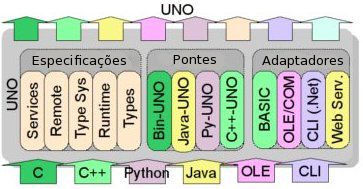
\includegraphics[scale=0.55,bb=0 0 510 180]{Uno-Arc.png}
\caption{Arquitetura do UNO. Adaptado de: \cite{uno_page}.}
\label{fig:uno_picture}
\end{figure}

A sessão seguinte apresenta uma biblioteca implementada em Python para utilizar o UNO nesta linguagem.

\subsection{PyUNO}
A biblioteca PyUNO permite que toda a API do OpenOffice.org seja utilizada na linguagem de programação Python de formas diferentes, como por exemplo utilizar \textit{scripts} executáveis em Python e através do \textit{framework} de \textit{scripts} do OpenOffice.org. A biblioteca não contém métodos que acessam o UNO, visto que toda implementação do UNO é carregada no Python \cite{pyuno_page}. Isto faz com que todo uso dos componentes seja no Python, toda especificação esteja na IDL e toda implementação no próprio UNO.

A subseções seguintes apresentam formas de utilização desta biblioteca.

\subsubsection{Python \textit{Scripts}}
\textit{Scripts} em Python são executáveis que se conectam ao OpenOffice.org utilizando o UNO. De todas maneiras possíveis, a utilização de \textit{scripts} é a forma mais lenta de uso, pois toda transferência é feita via conexão de rede. Como são implementados em Python, os \textit{scripts} são independentes do OpenOffice.org. A Figura \ref{pyuno.png} mostra como é executado um Python \textit{script}.
\begin{figure}[ht]
\centering
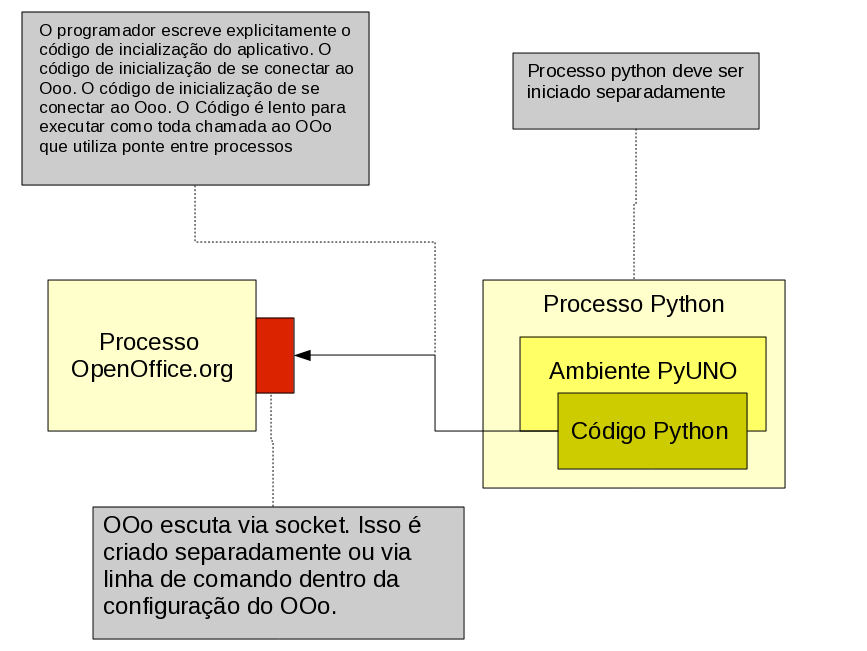
\includegraphics[scale=0.45,bb=0 0 634 460]{pyuno2.png}
\caption{\textit{Scripts} Python Utilizando PyUno. Adaptado de: \cite{web:uno}.}
\label{pyuno.png}
\end{figure}

Analisando a Figura \ref{pyuno.png} percebe-se que parte do código em Python é executado dentro do ambiente do PyUNO. Estes códigos são chamadas à API do UNO para criação dos componentes e a outra parte do código faz uso ou não destes objetos. Um exemplo de uso dos componentes do UNO é a criação do objeto que faz conexão ao processo OpenOffice.org.

\subsubsection{\textit{Script} Python como componente UNO}

Desta forma, os Python \textit{scripts} são implementados para serem inseridos dentro do OpenOffice.org, com isso há um ganho de desempenho pois não há necessidade de fazer conexão entre o processo OpenOffice.org e o Python \textit{script}. A Figura \ref{mode_component.png} mostra como o componente trabalha dentro de um processo OpenOffice.org.

\begin{figure}[ht]
  \centering
  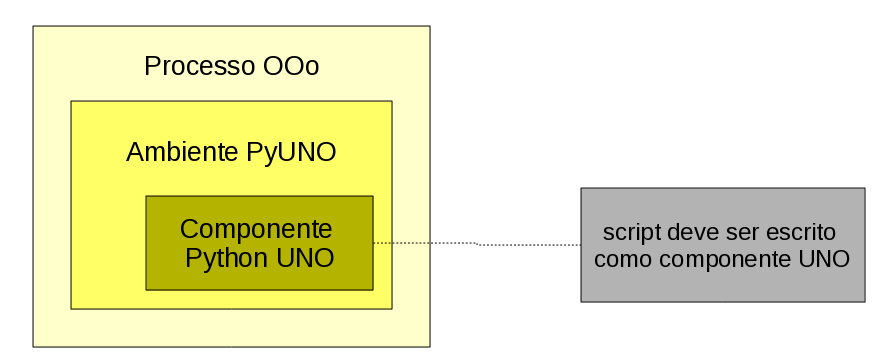
\includegraphics[scale=0.41,bb=0 0 574 257]{mode_component2.png}
  \caption{\textit{Scripts} Python como componente UNO. Adaptado de: \cite{web:uno}.}
\label{mode_component.png}
\end{figure}

\section{XML}

Segundo, \cite{xml_dummies}, XML é uma linguagem de marcação que utiliza \textit{tags} para rotular, categorizar e organizar as informações de maneira específica. A marcação descreve o documento ou a organização do mesmo. O conteúdo, como textos, imagens e dados, são partes do código que as \textit{tags} de marcação contêm. Além disso, o XML não está limitado a um conjunto especifíco de marcações, estas podem ser criadas para atender às necessidades, como exemplo a Figura \ref{xml.png} demonstra a criação de novas \textit{tags} de marcação para representar alunos.

\begin{figure}[ht]
\centering
\begin{center}
   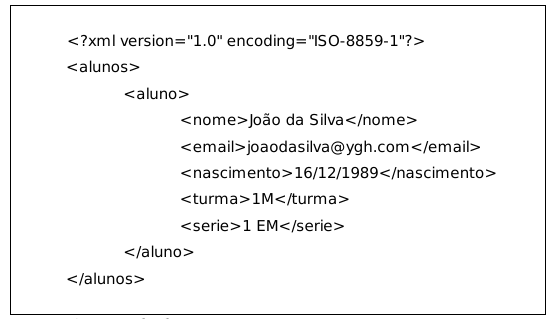
\includegraphics[scale=0.55,bb=0 0 450 236]{xml.png}
\end{center}
\caption{Exemplo de Arquivo XML. Fonte: \cite{ronaldo}.}
\label{xml.png}
\end{figure}

Pode ser notado na Figura \ref{xml.png}, a própria estrutura e declaração das \textit{tags} do XML declaram o conteúdo do documento, facilitando a leitura dos dados através de outras linguagens de programação.

\section{WSGI}
\label{wsgi}
Historicamente o \textit{Web Service Gateway Interface}(WSGI) foi proposto em 2003 por Philip J. Eby e programadores Python. Esta proposta, segundo \cite{wsgi:website}, tinha objetivo de criar um caminho fácil de integrar diferentes aplicações Web e obter uma única aplicação final.

Python possui atualmente uma variedade de \textit{frameworks} para construção de aplicações Web, tais como Zope, Django, Twisted Web, entre outros. Essa variedade tem um lado positivo onde é possível escolher um \textit{framework} que atenda melhor as necessidades atuais do desenvolvedor. Mas por outro lado, a escolha do \textit{framework Web} irá limitar a seleção de serviços Web utilizáveis, e vice-versa.

Em contrapartida, embora a linguagem de programação Java tenha também uma variedade de \textit{frameworks} disponíveis para construção de aplicações Web, esta tem a Java Servlet API que torna possível que aplicações desenvolvidas em qualquer \textit{framework Web} Java rode em qualquer servidor Web que suporta a API do \textit{servlet}.

Com a possibilidade de qualquer servidor Web rodar qualquer aplicação Web, tem-se o desenvolvimento independente da escolha do servidor Web. Além disso, deixa livre os desenvolvedores para escolherem o que melhor os atendam e se concentrar em sua área de especialização, deixando para outro desenvolvedor a responsabilidade de escolher qual servidor Web utilizar.

Em suma, esta proposta tenta resgatar a independência de aplicações e servidores Web como o Java Servlet API, para que facilite a escolha da tecnologia a ser utilizada tanto no desenvolvimento da aplicação quanto na ferramenta servidora.

\section{\textit{Web Service}}

Existem diferentes maneiras de definir um \textit{Web Service}. \citeonline{w3c}  define \textit{Web Service} como:
\begin{quote}
\textit{Um software projetado para suportar interações interoperáveis entre máquinas sobre uma rede. Tem uma interface descrita em um formato processável por máquina(especificamente WSDL). Outros sistemas interagem com este serviço Web de uma maneira prescrita usando mensagens SOAP, tipicamente transmitida usando HTTP com serialização XML em conjunto com outras normas relacionadas à Web.}
\end{quote}

\textit{Simple Object Acess Protocol}(SOAP), citado por \cite{w3c}, é um protocolo baseado em XML para troca de informações entre computadores, tendo seu foco principal a chamada de procedimentos remotos transportados via HTTP \cite{ethan}. Portanto, permitem que aplicativos cliente possam facilmente conectar-se a serviços remotos e invocar metódos. 

\textit{Web Service Description Language}(WSDL), também citado por \cite{w3c}, é um formato XML para descrever serviços de rede como um conjunto de parâmetros operacionais sobre as mensagens que contenham qualquer informação ou documento orientado para processo de orientação. As operações e mensagens são descritas abstratamente e estão ligado a um protocolo de rede concreto e formato de mensagem para definir um ponto de extremidade \cite{wsdl}.

Em outras palavras, é uma solução utilizada na integração de sistemas e na comunicação entre aplicações de diferentes arquiteturas \cite{book:webservice}, como demonstra a Figura \ref{imagem:webservice}.

\begin{figure}[ht]
 \centering
 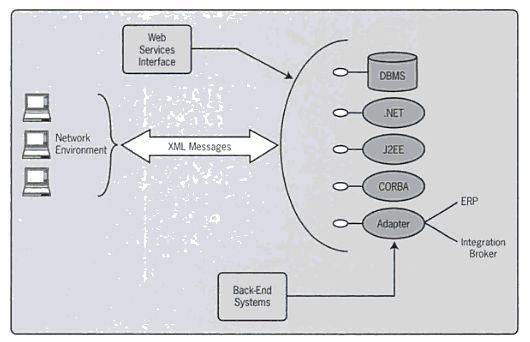
\includegraphics[scale=0.80,bb=0 0 450 250]{webservice_exemplo.png}
 \caption{Serviço Web com sistemas internos de plataformas diferentes, Adaptado de: \cite{webservice_foto}.}
\label{imagem:webservice}
\end{figure}

Note que na Figura \ref{imagem:webservice}, os clientes enxergam a aplicação como um sistema único e utilizam o mesmo protocolo de comunicação. Com isso, há uma independência tanto do cliente quanto do servidor, permitindo que estes exerçam o seu papel da melhor maneira possível.

Segundo \cite{ethan} e \cite{naveen}, existem três papéis principais dentro da arquitetura de serviços Web:
\begin{itemize}
 \item Prestador de Serviço - Fornece os serviços através da Web e responde os pedidos dos consumidores;
 \item Consumidor de Serviço - Utiliza uma rede existente através da abertura de uma conexão de rede e envia uma solicitação em XML. Em serviços Web baseados em SOAP, o prestador de serviço publica o contrato(WSDL) do serviço através da internet e o consumidor pode acessá-lo diretamente ou buscar o registro de serviço;
 \item Registro de Serviço - Diretório lógico centralizado de serviços onde os desenvolvedores podem publicar ou encontrar novos serviços já existentes, portanto, serve como uma agência centralizada para as empresas e seus serviços.
\end{itemize}

Com esta arquitetura flexível, um \textit{Web Service} pode ser um caminho para expansão dos negócios de uma empresa, com o objetivo de aumentar a eficiência do processo de negócio e sua experiência com o cliente, já que este não está limitado à automatização dos processos \cite{singh}. Além disso, pode simplificar as interações com serviços externos, tais como validação do cartão de crédito ou compra com o mesmo. Como resultado, são oferecidos aos clientes uma experiência enriquecida, com mais opções de escolha e mais flexibilidade. 

Com isso, cada \textit{Web service} é responsável por um processo, ou seja, cada aplicação tem a sua responsabilidade. Por exemplo um sistema que controla usuário e senha em um caixa eletrônico, é responsável somente autenticar usuários. Logo, tendo poucas atribuições ao serviço faz-se o uso do mesmo com mais rapidez e clareza.

\section{XML-RPC}
Segundo \cite{laurent}, XML-RPC é um dos métodos mais simples de serviços Web, e que torna fácil computadores chamarem procedimentos de outros computadores. Este método permite que programas façam chamadas de função ou procedimento em uma rede utilizando o protocolo \textit{Hypertext Transfer Protocol}(HTTP) para transferir informações de um computador cliente a um computador servidor. É utilizado a linguagem XML tanto para fazer requisições pelo cliente quanto para responder a ele. A Figura \ref{xmlrpc.jpg} apresenta como é a comunicação e a transferência das informações entre cliente e servidor.

\begin{figure}[ht]
 \centering
 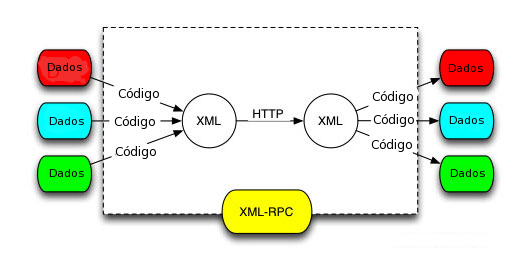
\includegraphics[scale=0.50,bb=0 0 550 250]{xmlrpc.jpg}
 \caption{Troca de mensagens utilizando XML-RPC, Adaptado de Fonte: \cite{web:xmlrpc}.}
\label{xmlrpc.jpg}
\end{figure}

Em uma arquitetura cliente-servidor, todos procedimentos são requisitados pelo cliente e executados pelo servidor. Para que isto seja possível utiliza-se uma das tecnologias de comunicação entre processos, a \textit{Remote Procedure Call}(RPC). RPC permite a um programa de computador chamar um procedimento no mesmo computador ou em outro conectado por uma rede. No caso do XML-RPC todas as chamadas são feitas através de uma rede de computadores mas para o RPC não existe diferença entre o procedimento estar na mesma máquina ou em outro computador.

\section{ERP}
\textit{Enteprise Resource Planning}(ERP) é um sistema de informação usado para gerenciar os recursos internos e externos de uma corporação \cite{wiki:erp}. Sua arquitetura tem como objetivo a facilidade de gestão do fluxo de informações, sendo este gerado pela integração dos dados e processos de vários ou mesmo da totalidade dos departamentos da organização num único sistema. Esta integração pode ser efetuada ao nível departamental ou funcional (sistemas finanças, marketing, comercial, pessoal, produção, etc.) ou ao nível processual(sistema de tratamento de encomendas, sistema de informação de gestão, sistema de apoio à decisão, etc.) \cite{557044}. 

Resumidamente, segundo \cite{557044}, ERP é uma tecnologia de suporte de software que forma um núcleo de processamento de transações, tendo sua aplicação em várias áreas.

\section{ERP5}

Para \cite{artigo:rogerio}, o ERP5 é um ERP de código aberto que visa oferecer uma solução de alta tecnologia e baixo custo, sendo desenvolvida pela Nexedi, criadora do software, e instituições de pesquisa de países da Europa e do Brasil. Este software é desenvolvido na plataforma Zope, escrito na linguagem de programação Python. O Zope é um servidor de aplicações Web de código aberto desenvolvido em Python \cite{python_zope} que oferece um banco de dados orientado a objeto(ZODB) e um máquina de estado(DC Workflow). Com isso, além de utilizar os recursos oferecidos pela plataforma, o ERP5 incorpora a sicronização entre diferentes bancos de dados orientado a objeto e um mecanismo de mapeamento de banco de dados relacional que indexa atributos de cada objeto em um banco de dados relacional \cite{handbook}.

\subsection{\textit{Business Templates}}
\textit{Business Templates} é a utilização de componentes existentes no ERP5 para adicionar novas funcionalidades ao núcleo do ERP5. Em outras palavras, a partir da reutilização dos recursos, campos e \textit{scripts}, é possível criar modelos de negócio utilizando componentes já existentes \cite{beautiful}.

\section{Buildout}

Buildout é uma ferramenta, desenvolvida em Python, que fornece suporte para criação de aplicações, seja ela desenvolvida em Python ou em outra linguagem de programação \cite{jim}. Entre vários mecanismos de criação e instalação de aplicações que o Buildout utiliza, os \textit{recipes} são os mais utilizados. \textit{Recipes} são \textit{scripts} Python que executam algum procedimento específico e possuem todas as informações do Buildout que está executando-o. A Figura \ref{buildout.png} é um exemplo de um arquivo de configuração do Buildout. 

\begin{figure}[ht]
 \centering
 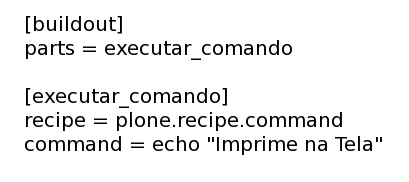
\includegraphics[scale=0.50,bb=0 0 550 250]{buildout.png}
 \caption{Arquivo de configuração do Buildout.}
\label{buildout.png}
\end{figure}

Na organização do arquivo de configuração, existem dois atributos importantes no buildout que são: \textit{parts}, \textit{recipe}. O \textit{parts} é utilizado para declarar qual procedimento será chamado. Dentro da declaração do procedimento tem o atributo \textit{recipe} que por sua vez é o caminho do script que executará todo procedimento. Por fim, na Figura \ref{buildout.png} temos além da declaração dos atributos essenciais, temos um atributo \textit{command}. Este atributo será utilizado pelo \textit{recipe} que foi implementado para executar o que estiver dentro do \textit{command}.

Em suma, o Buildout é extremamente flexível e simples para criação de ambientes de desenvolvimento específicos e enxutos.
 
\section{Subversion}

Segundo \cite{975530}, Subversion é um sistema de controle de versão de código aberto. Sistemas de controle de versão são utilizados em ambientes de desenvolvimento de software para controlar diferentes versões do código-fonte e possibilitar o trabalho em equipe. Para que isto ocorra, é fornecido pelo sistema um local centralizado para armazenamentos dos arquivos do projeto e sua revisões \cite{1197991}. Com isso, cada desenvolvedor pode utilizar uma revisão específica sem que outros desenvolvedores sejam afetados.